\section{Esempio di istogramma sperimentale}

\subsection{Introduzione}
In questo esempio, verranno presentati i dati di un esperimento di misura fisica, la fisica sottostante e il processo per creare un istogramma che rappresenti questi dati utilizzando il linguaggio di programmazione Python con la libreria Matplotlib.

\subsection{Descrizione dell'esperimento}
L'esperimento consiste nel misurare la lunghezza di un campione di barre metalliche. Le misure sono state effettuate utilizzando un calibro digitale con una precisione di 0.1 mm. Di seguito sono riportati i dati sperimentali ottenuti (in cm):

\[
\begin{array}{cccccc}
45.1 & 47.2 & 49.3 & 50.5 & 52.6 & 54.7 \\
48.3 & 46.9 & 51.2 & 53.8 & 50.0 & 49.9 \\
48.7 & 51.5 & 52.1 & 47.6 & 46.3 & 50.9 \\
51.8 & 48.0 & 49.5 & 50.3 & 47.0 & 46.5 \\
52.4 & 48.8 & 49.2 & 51.3 & 47.8 & 50.7 \\
\end{array}
\]
Nel contesto della statistica, useremo solo programmi software e ci disinteresseremo dei problemi relativi alle cifre significative durante i calcoli, mentre queste saranno importanti nel momento in cui scriveremo il risultato delle misure.
\subsection{Fisica dell'esperimento}
La misura della lunghezza delle barre metalliche è un esperimento comune in fisica per studiare le proprietà dei materiali. La lunghezza può variare a causa di fattori come:
\begin{itemize}
    \item Differenze nel processo di produzione.
    \item Espansione termica a diverse temperature.
    \item Errori sistematici e casuali durante la misurazione.
\end{itemize}
L'istogramma delle misure permette di visualizzare la distribuzione delle lunghezze e di identificare eventuali deviazioni significative dalla media.

\subsection{Creazione dell'istogramma con Python}
Per creare l'istogramma, utilizziamo il seguente codice Python:

\begin{lstlisting}[language=Python, caption=Codice Python per creare l'istogramma]
import matplotlib.pyplot as plt

# Dati sperimentali
dati_sperimentali = [45.1, 47.2, 49.3, 50.5, 52.6, 54.7, 48.3, 46.9, 51.2, 53.8, 
                     50.0, 49.9, 48.7, 51.5, 52.1, 47.6, 46.3, 50.9, 51.8, 48.0, 
                     49.5, 50.3, 47.0, 46.5, 52.4, 48.8, 49.2, 51.3, 47.8, 50.7]

# Crea l'istogramma
plt.figure(figsize=(10, 6))
plt.hist(dati_sperimentali, bins=8, edgecolor='black', alpha=0.7)

# Aggiungi titolo e etichette
plt.title('Istogramma dei dati sperimentali')
plt.xlabel('Misura (cm)')
plt.ylabel('Frequenza')

# Mostra l'istogramma
plt.savefig('istogramma2.png')  # Salva l'immagine come istogramma2.png
#se vuoi scaricare il file da google colab decommenta le righe:
#from google.colab import files
#files.download('istogramma2.png')
plt.show()
\end{lstlisting}

\subsubsection{Spiegazione del codice}
Il codice Python utilizzato per creare l'istogramma è spiegato di seguito:

\paragraph{Importazione delle librerie}
\begin{lstlisting}[language=Python, caption=Importazione delle librerie]
import matplotlib.pyplot as plt
\end{lstlisting}
Questo codice importa la libreria Matplotlib, necessaria per la creazione di grafici.

\paragraph{Definizione dei dati}
\begin{lstlisting}[language=Python, caption=Definizione dei dati]
dati_sperimentali = [45.1, 47.2, 49.3, 50.5, 52.6, 54.7, 48.3, 46.9, 51.2, 53.8, 
                     50.0, 49.9, 48.7, 51.5, 52.1, 47.6, 46.3, 50.9, 51.8, 48.0, 
                     49.5, 50.3, 47.0, 46.5, 52.4, 48.8, 49.2, 51.3, 47.8, 50.7]
\end{lstlisting}
Definisce un array contenente i dati delle misurazioni fisiche.

\paragraph{Creazione dell'istogramma}
\begin{lstlisting}[language=Python, caption=Creazione dell'istogramma]
plt.figure(figsize=(10, 6))
plt.hist(dati_sperimentali, bins=8, edgecolor='black', alpha=0.7)
\end{lstlisting}
Imposta la dimensione della figura e crea un istogramma con 8 bin, bordi neri per i bin e trasparenza del 70\%.

\paragraph{Aggiunta di titolo e etichette}
\begin{lstlisting}[language=Python, caption=Aggiunta di titolo e etichette]
plt.title('Istogramma dei dati sperimentali')
plt.xlabel('Misura (cm)')
plt.ylabel('Frequenza')
\end{lstlisting}
Aggiunge il titolo e le etichette agli assi del grafico.

\paragraph{Visualizzazione e salvataggio dell'istogramma}
\begin{lstlisting}[language=Python, caption=Visualizzazione e salvataggio dell'istogramma]
plt.savefig('istogramma2.png')  # Salva l'immagine come istogramma2.png
plt.show()
\end{lstlisting}
Visualizza l'istogramma generato e lo salva come `istogramma2.png`.

\subsection{Risultati}
L'istogramma risultante mostra la distribuzione delle lunghezze delle barre metalliche. L'analisi visiva dell'istogramma permette di identificare la variabilità delle misurazioni e la presenza di eventuali outlier.

\begin{figure}[!htbp] 
    \centering
    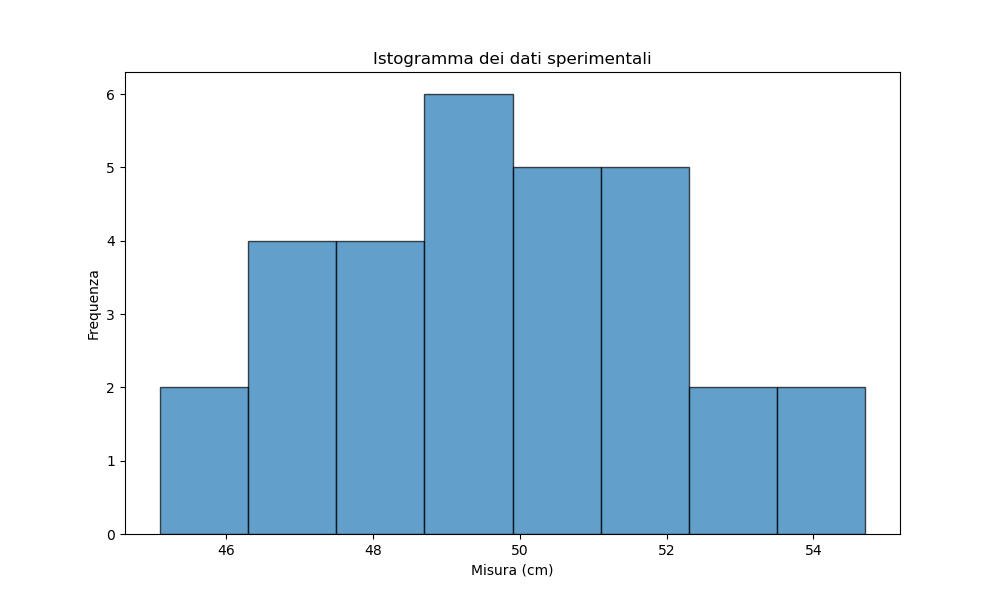
\includegraphics[width=0.8\textwidth]{istogramma2.png}
    \caption{Istogramma dei dati sperimentali}
    \label{fig:istogramma2}
\end{figure}



